\documentclass{article}

%----------------------------------------------------------------------------------------
%	PACKAGES AND OTHER DOCUMENT CONFIGURATIONS
\usepackage[utf8]{inputenc}
\usepackage{graphicx}
\usepackage{tabularx}
\usepackage[export]{adjustbox}
\usepackage{paralist}
\usepackage{wrapfig}
\usepackage{float}
\usepackage{geometry}
 \geometry{
 a4paper,
 total={170mm,257mm},
 left=20mm,
 top=20mm,
 }

%----------------------------------------------------------------------------------------
\newcommand*{\plogo}{\fbox{$\mathcal{PL}$}} % Generic publisher logo

%----------------------------------------------------------------------------------------
%	TITLE PAGE
%----------------------------------------------------------------------------------------

\newcommand*{\titleGP}{\begingroup % Create the command for including the title page in the document
\centering % Center all text
\vspace*{\baselineskip} % White space at the top of the page

\rule{\textwidth}{1.6pt}\vspace*{-\baselineskip}\vspace*{2pt} % Thick horizontal line
\rule{\textwidth}{0.4pt}\\[\baselineskip] % Thin horizontal line

{\LARGE Caracal Automated Marking \\ Software Requirements \\ Specification}\\[0.2\baselineskip]  % Title 

Version: (1.0.0) 


\rule{\textwidth}{0.4pt}\vspace*{-\baselineskip}\vspace{3.2pt} % Thin horizontal line
\rule{\textwidth}{1.6pt}\\[\baselineskip] % Thick horizontal line

\scshape % Small caps
\vspace*{2\baselineskip} % Whitespace between location/year and editors

Edited by \\[\baselineskip]
{\Large Oratile Motswagosele \\ Mankgwanyane Tlaka \\ Lesego Makaleng \\ Kenneth Mangwane \par} % Editor list

{\itshape University of Pretoria\par} % Editor affiliation

\begin{figure}[t]
\centering
	
\includegraphics[width=350px]{Images/UP_Logo}
\end{figure}

{\scshape 2017} \\[0.3\baselineskip] % Year published
{ Project Client: Caracal Research}\par % Publisher

\endgroup}

\begin{document}

\titleGP % This command includes the title page
\pagebreak

\clearpage
\tableofcontents
\clearpage

\section{Vision and Scope}
	\subsection{Project Background}
	
	\subsection{Project Vision}
	
	\subsection{Architecture Design}
		\subsubsection{Architectural Patterns}
		\subsubsection{Quality Requirements}
		\subsubsection{Architectural Tactics}
	
	\subsection{Project Scope}
	
\section{Modularization}
	\subsection{Access Module}
		\subsubsection{Scope}
			 The scope of this module will be to give users a graphical user interface, which will allow them to login/register and also to be able to have access to the system as whole.Access to the entire system will be made possible by making use of a request and render process , see the domain below. This module will be in charge of deploying a GUI on multiple browsers i.e. FireFox, Google Chrome, Microsoft Edge. Web browser will be the only supported access channel  and recommended devices will be limited to a desktop or laptop only. 
		
			 \begin{figure}[H]
			\centering
				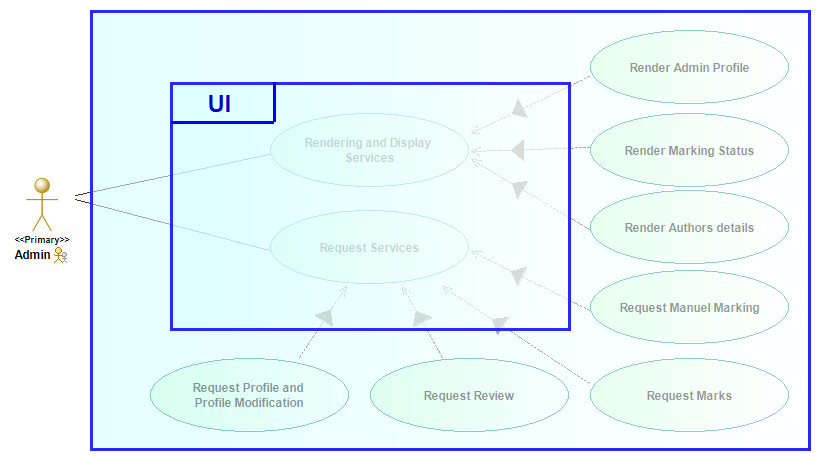
\includegraphics[width=450px]{Images/Access_Module/Pictures/Acess_Use_Case_Diagram_Scope}
			\end{figure}
		\subsubsection{Domain Model}
			\begin{figure}[H]
			\centering
				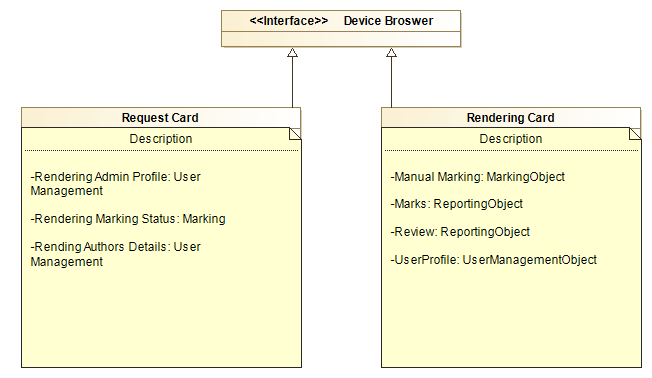
\includegraphics[width=450px]{Images/Access_Module/Pictures/Access_module_Class_diagram}
			\end{figure}
			
			\par The domain model above shows how the system will make use of a card system. where the user will be able 
			to interact with the entire system to the use of only interacting with one card at the time. The render 
			card will be be responsible to render and display all the functionality requested from the Request card.
		
			
		\subsubsection{Technologies}
			\paragraph{Programming Languages}
				\begin{enumerate}
 					 \item Python
 					 		Due to python's ability of being a general purpose language and both a scripting language
 					 		we will use it as a scripting language to connect to the server so that we will be able to
 					 		render requested functionality to the user.
  						\item PHP
  							\par PHP will be our main language for developing the website. mainly for its ability to be both 	
  							server side and client side, this will reduce number of different languages to be used.
  							
  							\par frameworks such as bootstrap will be used for the design of the 
  							layout of the user interface and human
  							computer interaction principles will be followed.
				\end{enumerate}
				
			\paragraph{Web Development Technologies}
				\paragraph{Symfony \newline}	
					 Symfony is a PHP web application framework and a set of reusable PHP components/libraries.
					Symfony aims to speed up the creation and maintenance of web applications and to 
					replace repetitive coding tasks.
					Symfony has a low performance overhead used with a bytecode cache.Symfony is aimed at building robust applications in an enterprise context, and aims to
					 give developers full control over the configuration: from the directory structure to the
					  foreign libraries, almost everything can be customized. To match enterprise
					   development guidelines, Symfony is bundled with additional tools to help developers test, debug 
					  and document project
					  
					  Symfony makes heavy use of existing PHP open-source projects as part of the framework, including:
					  \begin{itemize}
					  	\item Propel or Doctrine as object-relational mapping layers
					  	\item PDO database abstraction layer 
					  	\item PHPUnit, a unit testing framework
					  	\item Twig, a templating engine
					  	\item Swift Mailer, an e-mail library
					  \end{itemize}
					  
				

	\subsection{User Management Module}
		\subsubsection{Scope}
		\subsubsection{Domain Model}
		\subsubsection{Service Contracts}
		\subsubsection{Technologies}
		
	\subsection{Notifications Module}
		\subsubsection{Scope}
		\subsubsection{Domain Model}
		\subsubsection{Service Contracts}
		\subsubsection{Technologies}
		
	\subsection{Data Streaming and Security Module}
		\subsubsection{Scope}
		\subsubsection{Domain Model}
		\subsubsection{Service Contracts}
		\subsubsection{Technologies}

	\subsection{Marking Module}
		\subsubsection{Scope}
		\subsubsection{Domain Model}
		\subsubsection{Service Contracts}
		\subsubsection{Technologies}
		
	\subsection{Reporting Module}
		\subsubsection{Scope}
		\subsubsection{Domain Model}
		\subsubsection{Service Contracts}
		\subsubsection{Technologies}
		
	\subsection{I/O Module}
		\subsubsection{Scope}
		\subsubsection{Domain Model}
		\subsubsection{Service Contracts}
		\subsubsection{Technologies}
		
\end{document}
